\section{Tools}

\begin{frame}
\frametitle{Tools already discussed in Summer School}
\begin{itemize}
\item \href{https://minizinc.org}{MiniZinc}
\item \href{https://cpmpy.readthedocs.io}{CPMpy}
\item \href{https://github.com/ciaranm/glasgow-constraint-solver}{Glasgow Constraint Solver}
\end{itemize}
\end{frame}

\begin{frame}
\frametitle{Other Academic Solvers}
\begin{itemize}
\item Gecode (KTH, Sweden)
\item Choco-solver (IMT Atlantique, France)
\item MiniCP (Louvain, U Conn, Georgia Tech)
\item MaxiCP (Louvain, U Conn, Georgia Tech)
\item SICStus Prolog (RISE, Sweden) 
\end{itemize}
\end{frame}

\begin{frame}
\frametitle{Commercial Tools}
\begin{itemize}
\item \href{https://ibm.com}{CP Optimizer}
\begin{itemize}
\item P. Laborie et al, 2018: IBM ILOG CP optimizer for scheduling
20+ years of scheduling with constraints at IBM/ILOG
\end{itemize}

\item \href{https://developers.google.com}{CP-Sat}
\begin{itemize}
\item L. Perron et al, Invited Talk, CP 2023: The CP-SAT-LP Solver
\item \href{https://www.youtube.com/embed/vvUxusrUcpU?si=ldUAKR6WqdfAIrhL}{Video in Scheduling Seminar}
\end{itemize}

\item \href{https://optalcp.com}{OptalCP}
\begin{itemize}
\item P. Vilim, Invited Talk, CP 2023: CP Solver Design for Maximum CPU Utilization
\item \href{https://www.youtube.com/embed/1Dm-kY3ekKo?si=wn34td-NrpOxknB4}{Video in Scheduling Seminar}
\end{itemize}

\item \href{https://hexaly.com}{Hexaly}
\begin{itemize}
\item T. Benoist, Tutorial at CP 2026
\item \href{https://www.youtube.com/embed/VjB5FoaFFUM?si=27yxZJAfkEBroxZf}{Video in Scheduling Seminar}
\end{itemize}
\end{itemize}
\end{frame}

\section{Learning Materials}

\begin{frame}
\frametitle{Learning Materials}
\begin{itemize}
\item Workshops on Teaching CP at CP 2015, CP 2023 \url{https://hsimonis.github.io/WTCP2023/index.html}
\item Survey of teaching materials with Tejas Santanam (Georgia Tech)
\item Available at \url{https://arxiv.org/abs/2403.12717}
\end{itemize}
\end{frame}

\section{Companies}

\begin{frame}
\frametitle{IBM and Constraint Programming}
\begin{quote}
Constraint programming technology is used to find solutions to scheduling and combinatorial optimization problems. It is based primarily on computer science fundamentals, such as logic programming and graph theory, in contrast to mathematical programming, which is based on numerical linear algebra.

Constraint programming is invaluable when dealing with the complexity of many real-world sequencing and scheduling problems.
\end{quote}
IBM {\tiny (\url{https://ibmdecisionoptimization.github.io/docplex-doc/cp.html})}
\end{frame}

\begin{frame}
\frametitle{Examples}
\begin{itemize}
\item Cosling, France
\item OptalCP, France, Czech Republic
\item Hexaly, France
\item Keelvar, Ireland
\item Opturion, Australia
\item Optix Solutions, Hong Kong
\end{itemize}
\end{frame}

\begin{frame}
\frametitle{\href{https://www.cosling.com}{Cosling}}

\includegraphics[width=12cm]{images/cosling.png}
\end{frame}

\begin{frame}
\frametitle{\href{https://www.optalcp.com}{OptalCP}}
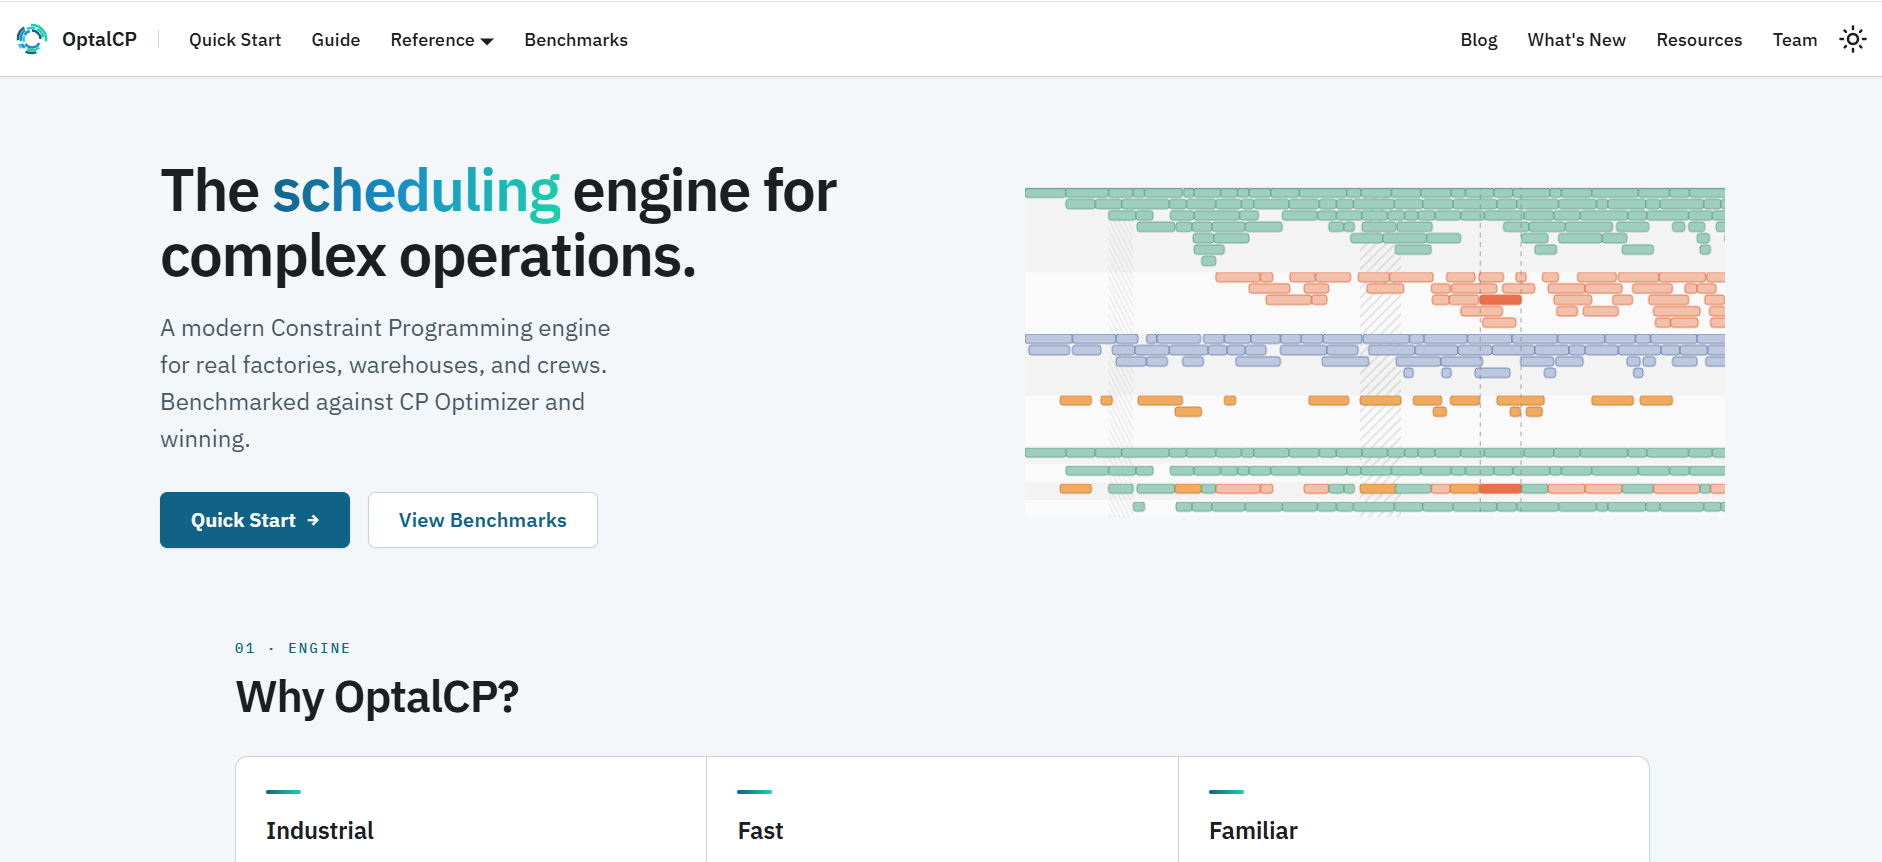
\includegraphics[width=12cm]{images/optalcp.png}
\end{frame}

\begin{frame}
\frametitle{\href{https://www.hexaly.com}{Hexaly}}
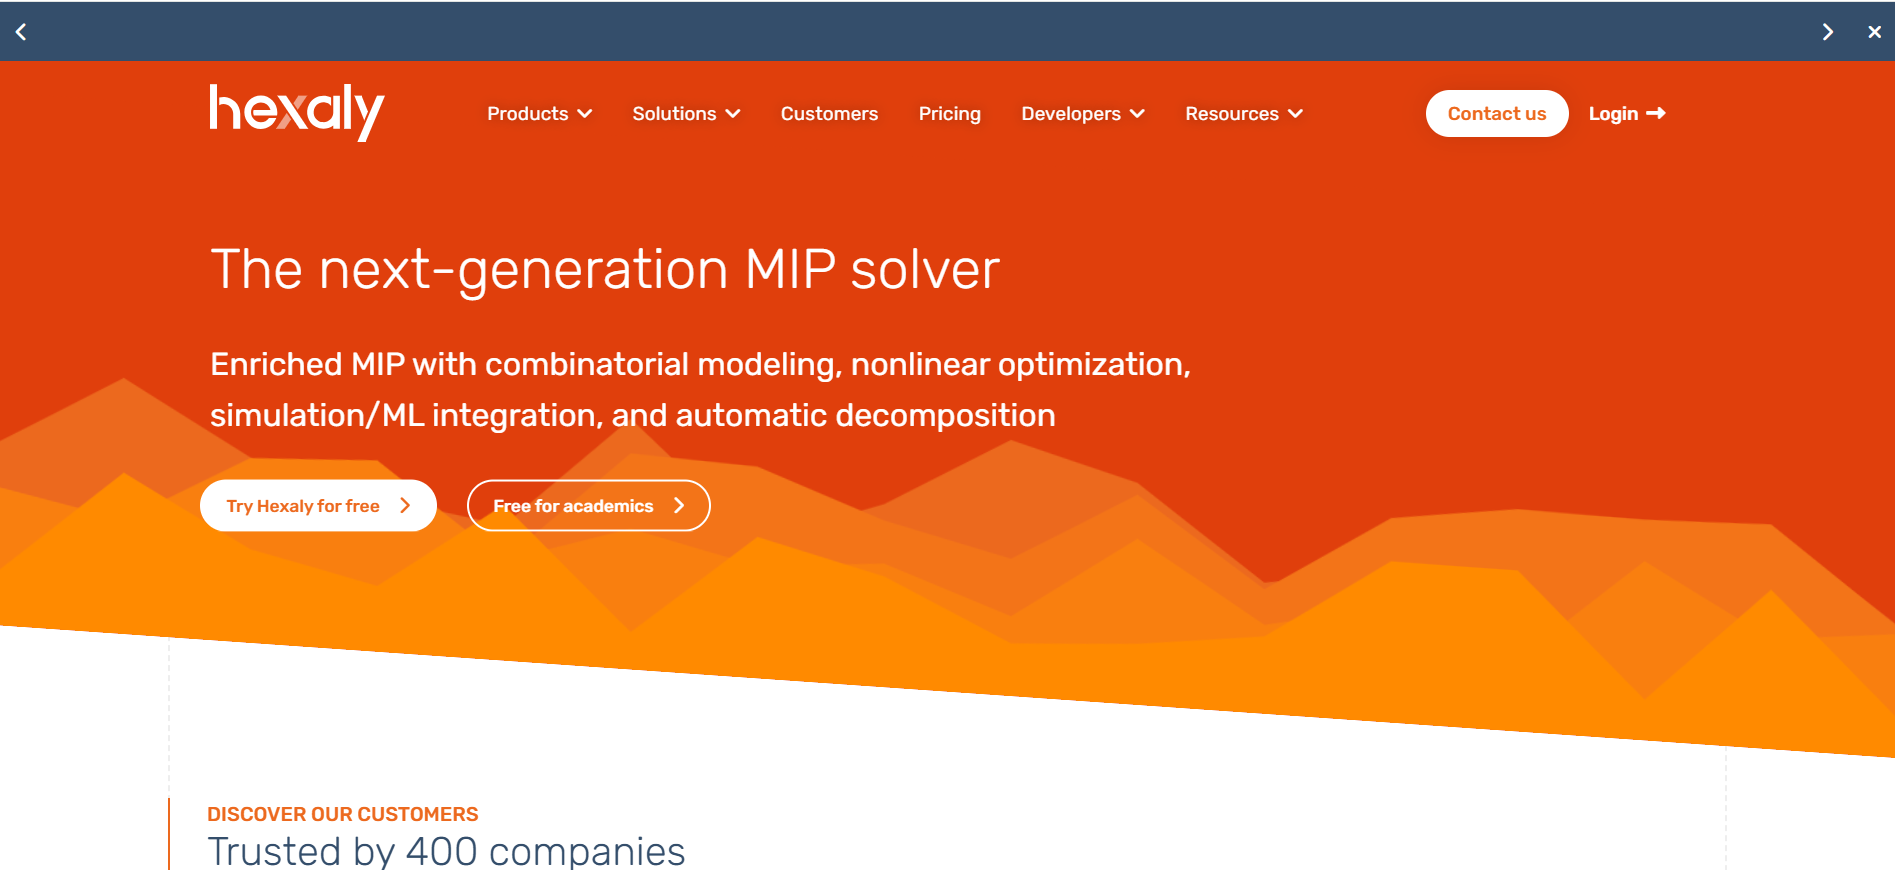
\includegraphics[width=12cm]{images/hexaly.png}
\end{frame}

\begin{frame}
\frametitle{\href{https://www.keelvar.com}{Keelvar}}

\includegraphics[width=12cm]{images/keelvar.png}
\end{frame}

\begin{frame}
\frametitle{\href{https://www.opturion.com}{Opturion}}

\includegraphics[width=12cm]{images/opturion.png}
\end{frame}

\begin{frame}
\frametitle{\href{https://www.optixsolutions.com.hk}{Optix Solutions}}

\includegraphics[width=12cm]{images/optixsolutions.png}
\end{frame}

\section{Literature Overview}

\begin{frame}
\frametitle{Literature Overview}
\begin{itemize}
\item Getting started in field can be overwhelming
\item A lot of work has been done
\item What is most relevant?
\item What is most related to what I want to do?
\item Where should I publish?
\item Getting to know the community
\end{itemize}
\end{frame}

\subsection{CP Conference}

\begin{frame}
\frametitle{CP Conference}
\begin{itemize}
\item Organised by Association for Constraint Programming (ACP)
\item Yearly since 1995
\item Special application track since 2002
\item CP 2027 will be here in Jilin
\item Survey of all papers since 2010 
\item Online version at \url{https://hsimonis.github.io/pthg24/cpconference.pdf}
\end{itemize}
\end{frame}

\begin{frame}
\frametitle{CP Conference Papers by Track}
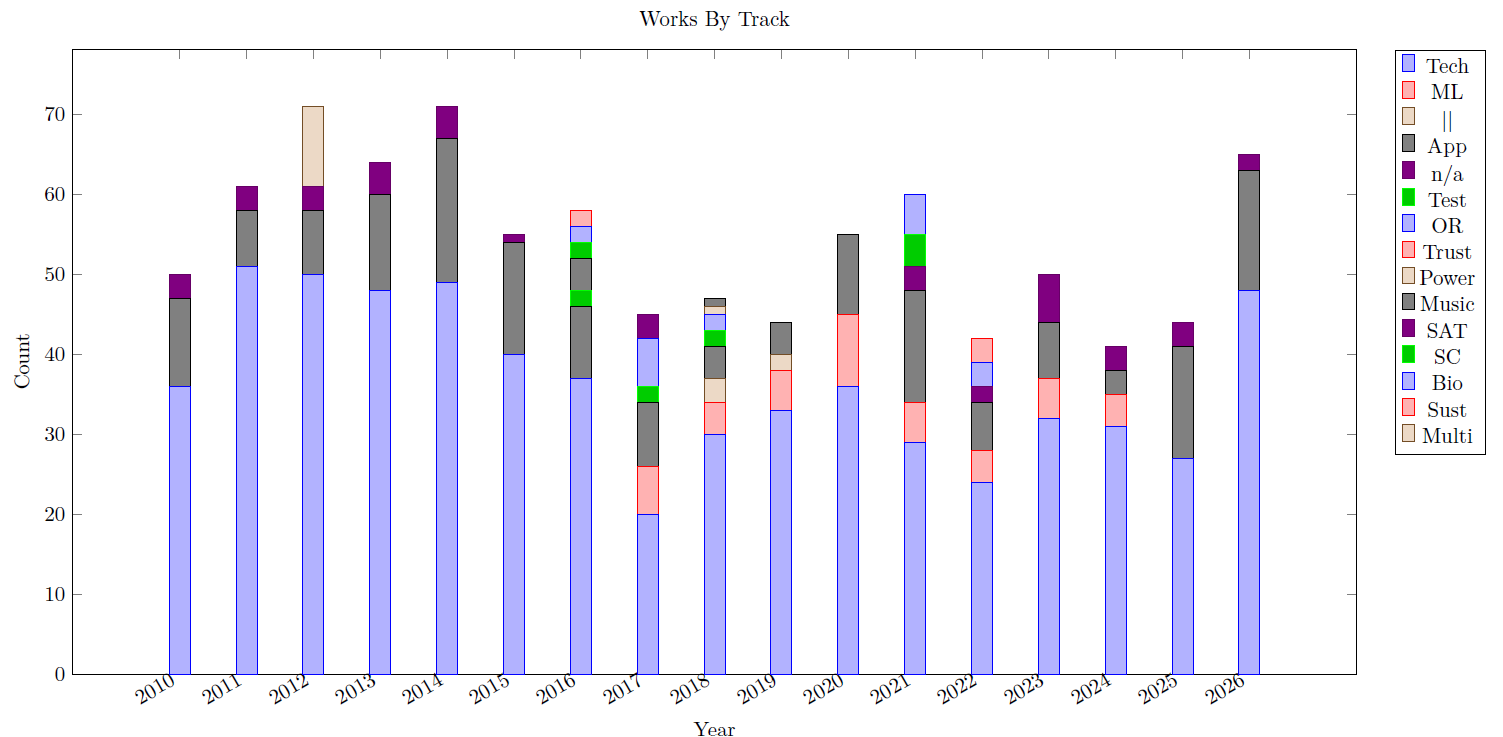
\includegraphics[width=12cm]{images/cpbytrack}
\end{frame}

\begin{frame}
\frametitle{CP Conference Award Winning Papers}
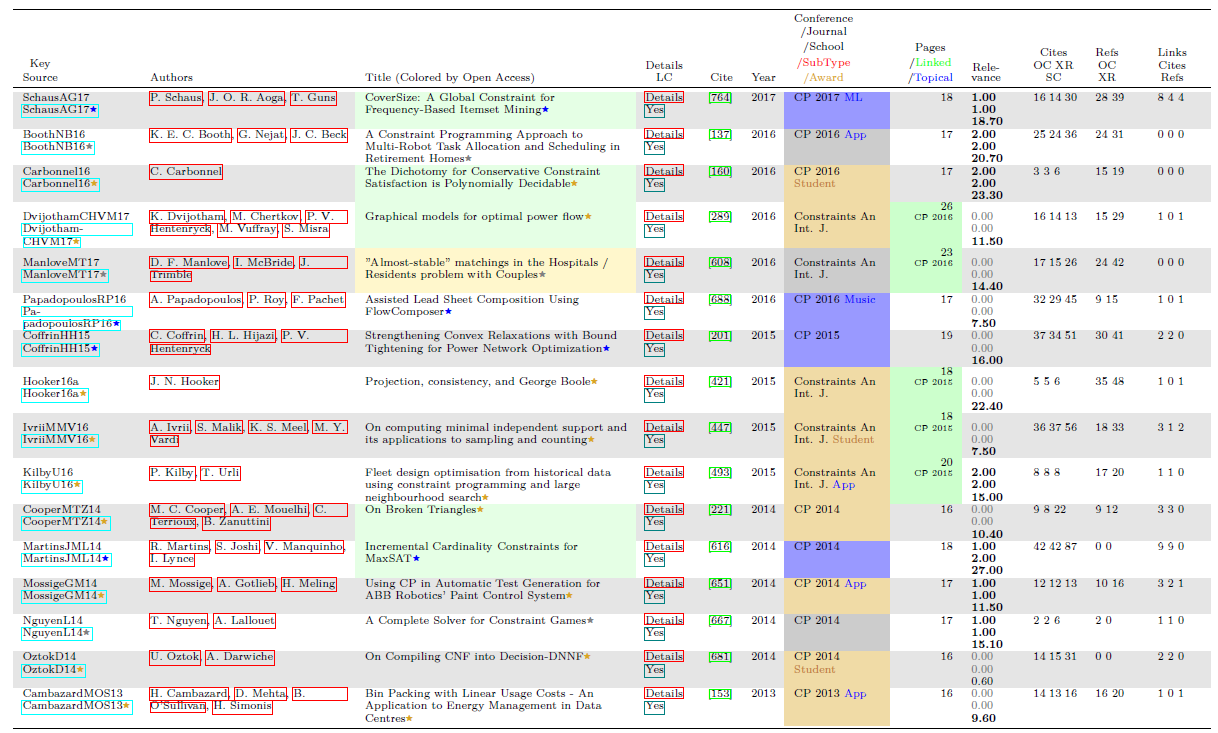
\includegraphics[width=12cm]{images/cpawardwinning}
\end{frame}

\begin{frame}
\frametitle{CP Conference Most Cited Papers}
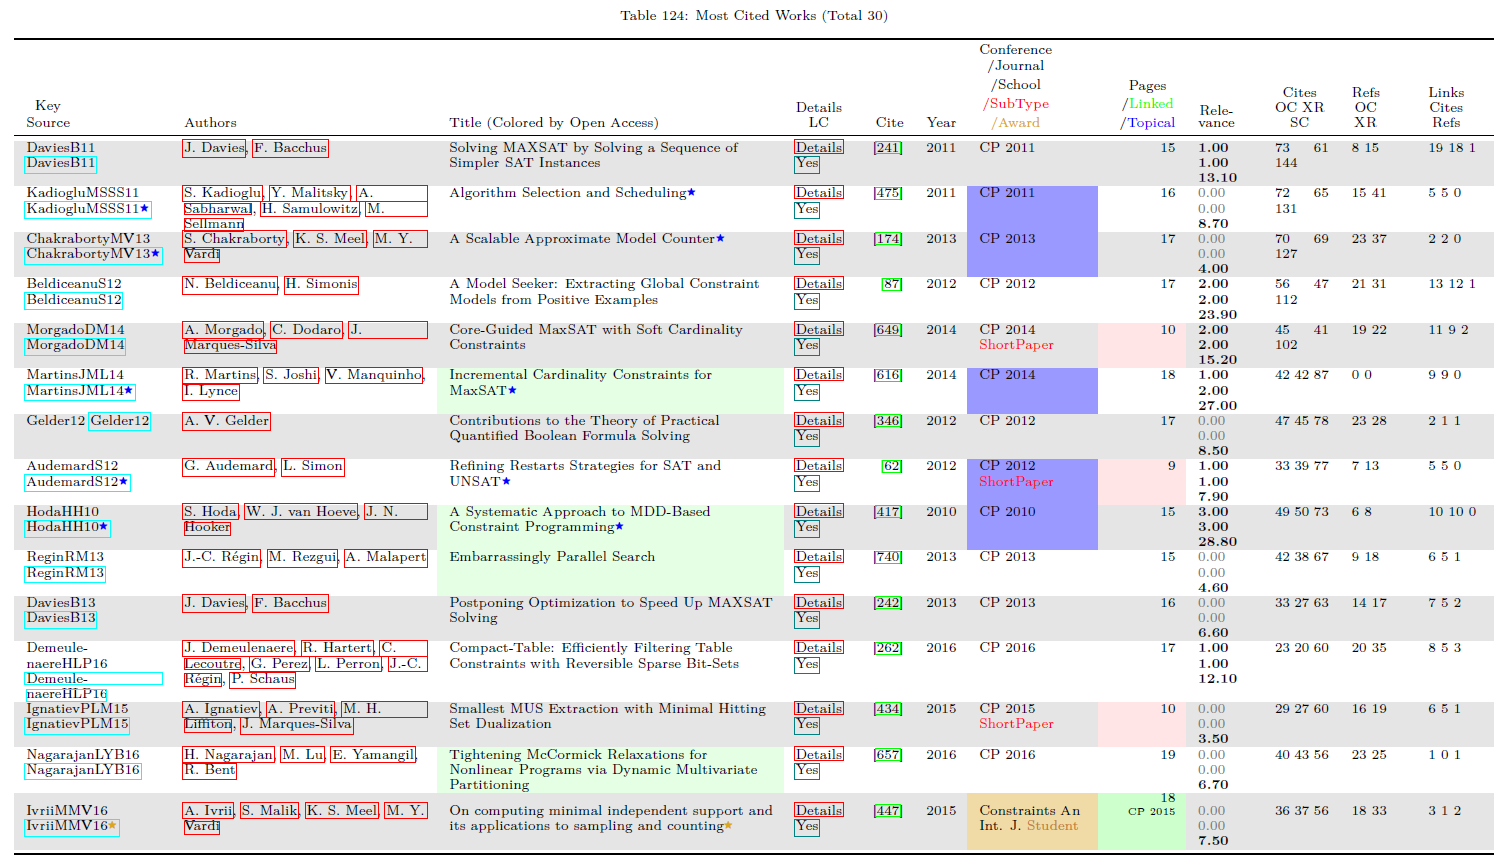
\includegraphics[width=12cm]{images/cpmostcited}
\end{frame}

\subsection{Constraints Journal}

\begin{frame}
\frametitle{Constraints Journal}
\begin{itemize}
\item Shameless plug by EiC (me)
\item Published by Springer
\item 30 years, started in 1996
\item Often publishes extended versions of CP/CPAIOR conference papers
\item Also longer form original articles
\item Submissions welcome!
\item Survey online version at \url{https://hsimonis.github.io/pthg24/constraints.pdf}
\item A data analysis at \url{https://hsimonis.github.io/pthg24/slidescp2026.pdf}
\end{itemize}
\end{frame}

\begin{frame}
\frametitle{Constraints Journal Articles by Country}
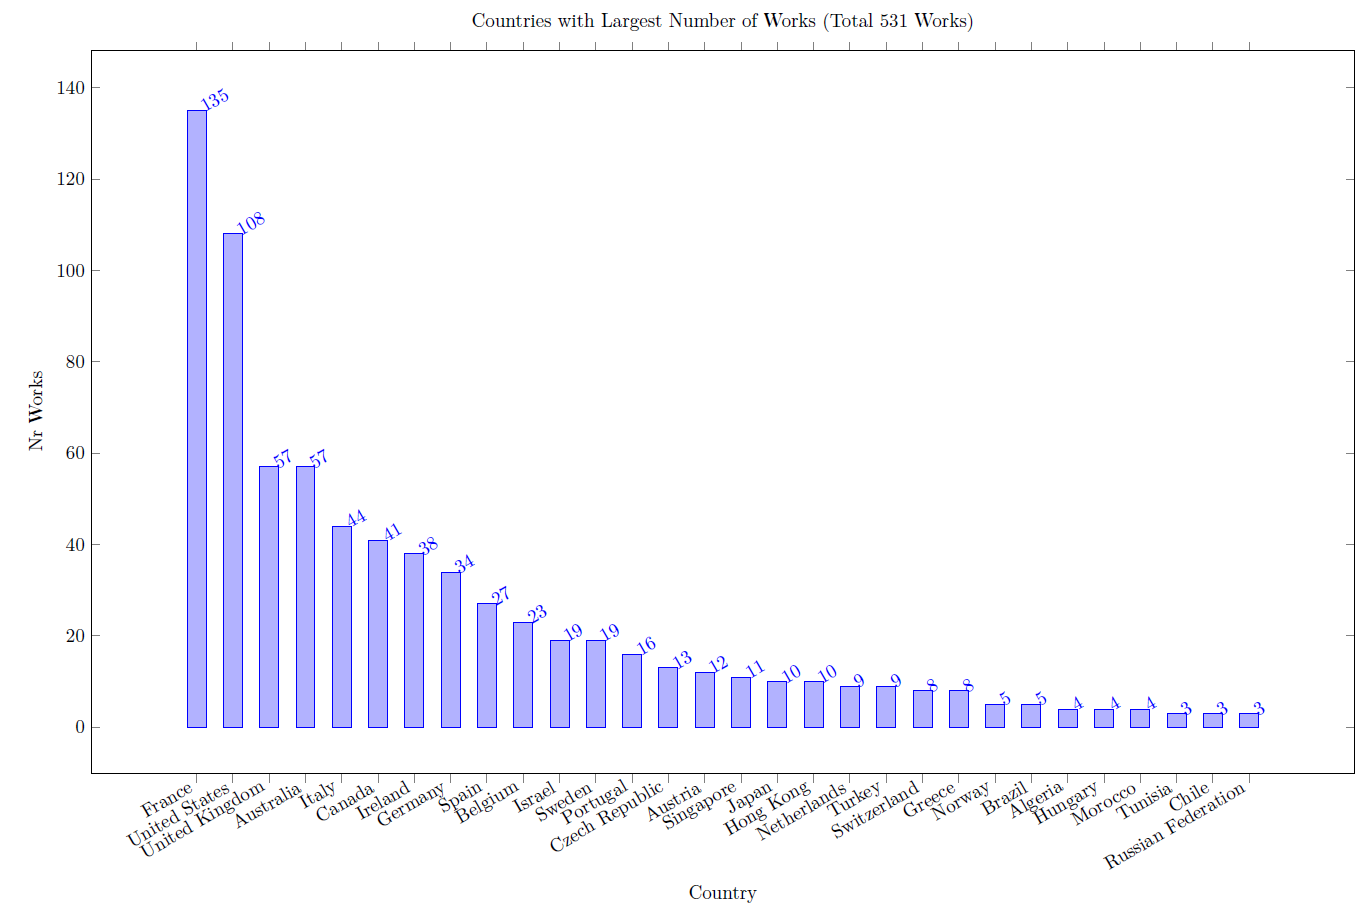
\includegraphics[width=11cm]{images/constraintscountry}
\end{frame}

\begin{frame}
\frametitle{Constraints Journal Citations}
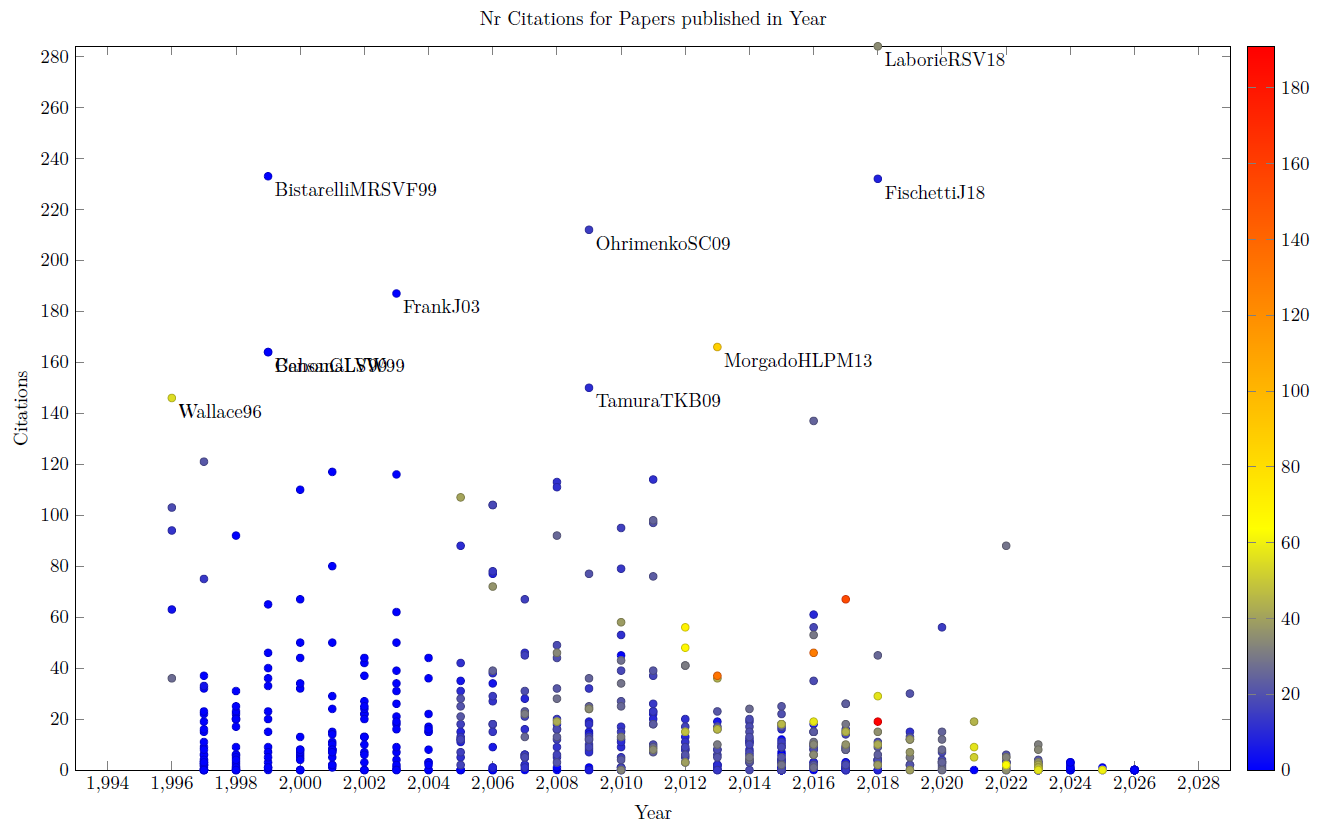
\includegraphics[width=11cm]{images/constraintscitations}
\end{frame}

\begin{frame}
\frametitle{Constraints Journal Special Issues}
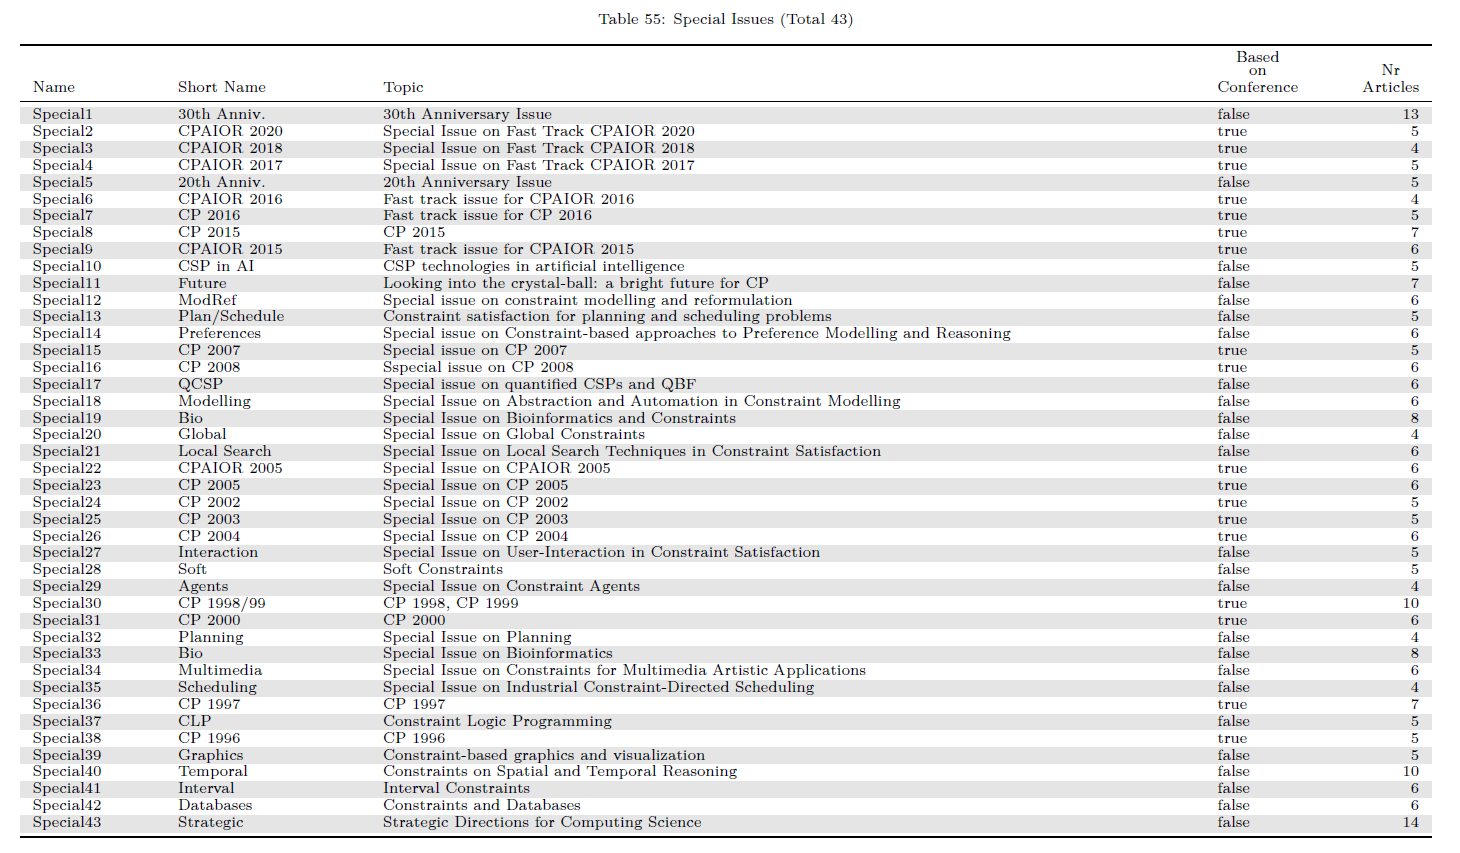
\includegraphics[width=12cm]{images/constraintsspecialissues}
\end{frame}



\subsection{CP and Scheduling}

\begin{frame}
\frametitle{}
\begin{itemize}
\item Joint work with Cemal Ozturk (MTU)
\item Overview of works combining CP with scheduling
\item Works since 1980
\item Survey online at \url{https://hsimonis.github.io/pthg24/scheduling.pdf}
\end{itemize}
\end{frame}

\begin{frame}
\frametitle{CP \& Scheduling Conferences}
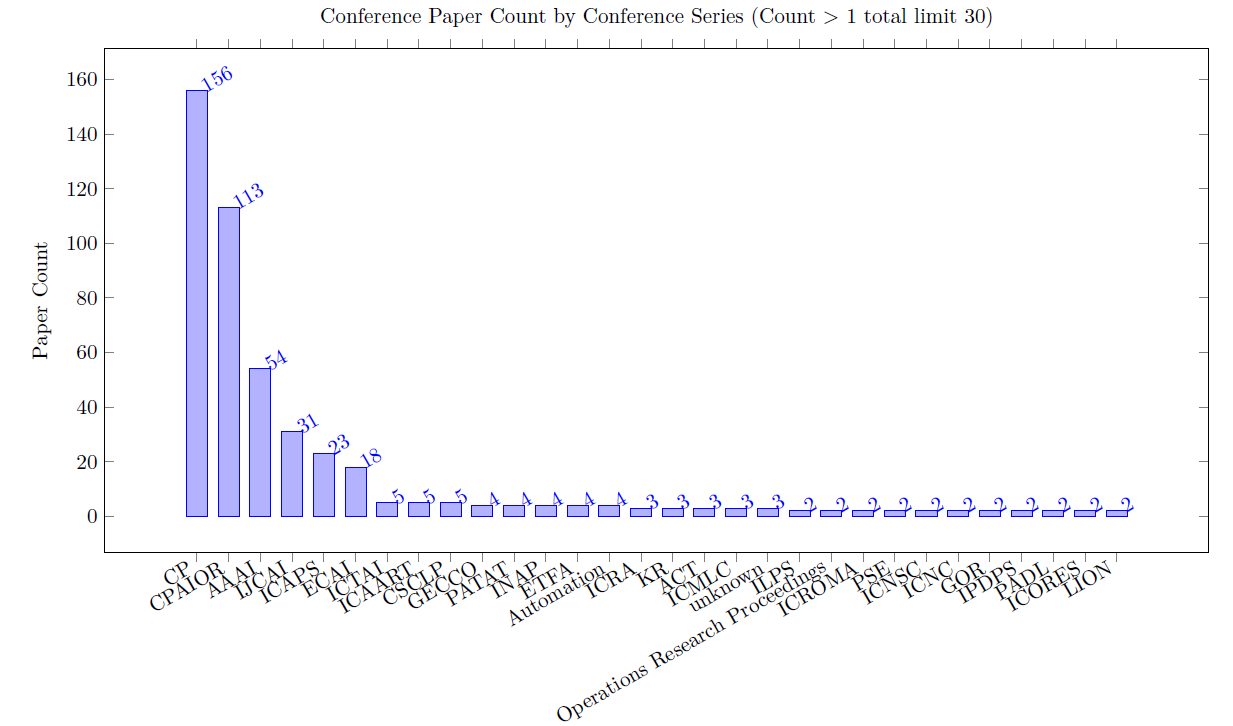
\includegraphics[width=12cm]{images/schedulingconferences}
\end{frame}

\begin{frame}
\frametitle{CP \& Scheduling Journals}
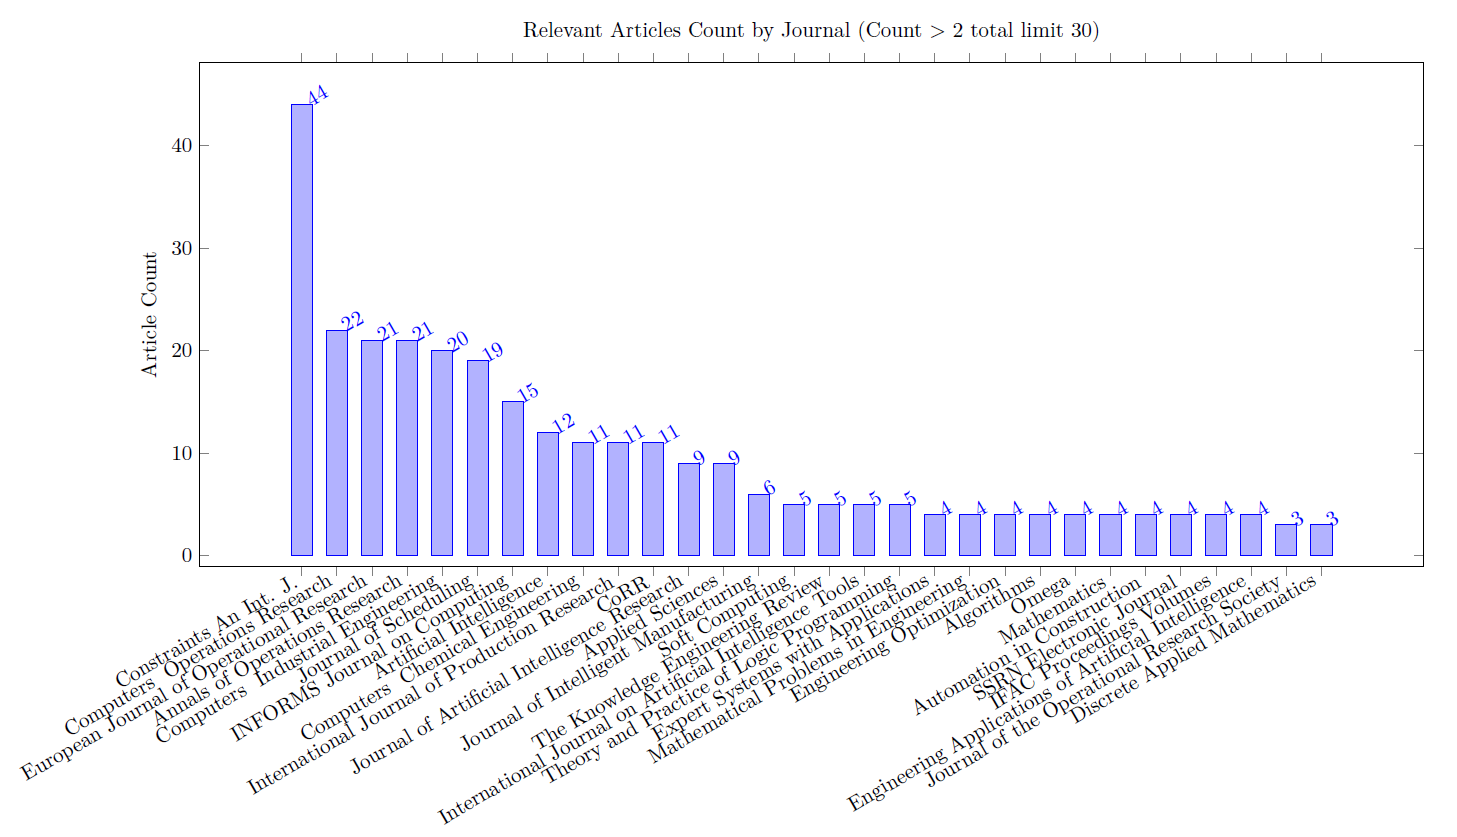
\includegraphics[width=12cm]{images/schedulingjournals}
\end{frame}

\begin{frame}
\frametitle{CP \& Scheduling Prolific Authors}
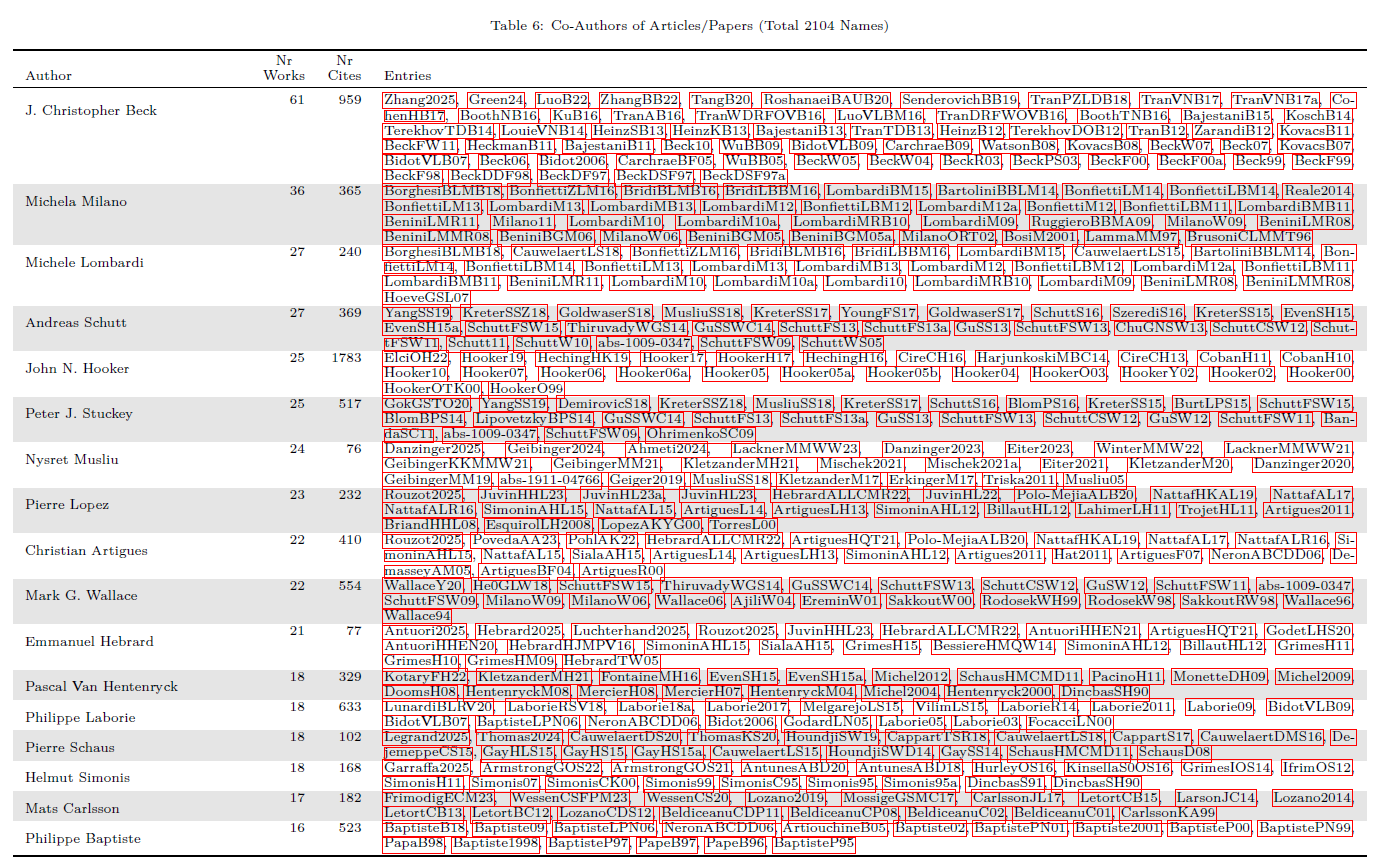
\includegraphics[width=11cm]{images/schedulingauthors}
\end{frame}

\begin{frame}
\frametitle{CP \& Scheduling Co-Author Graph (Excerpt)}
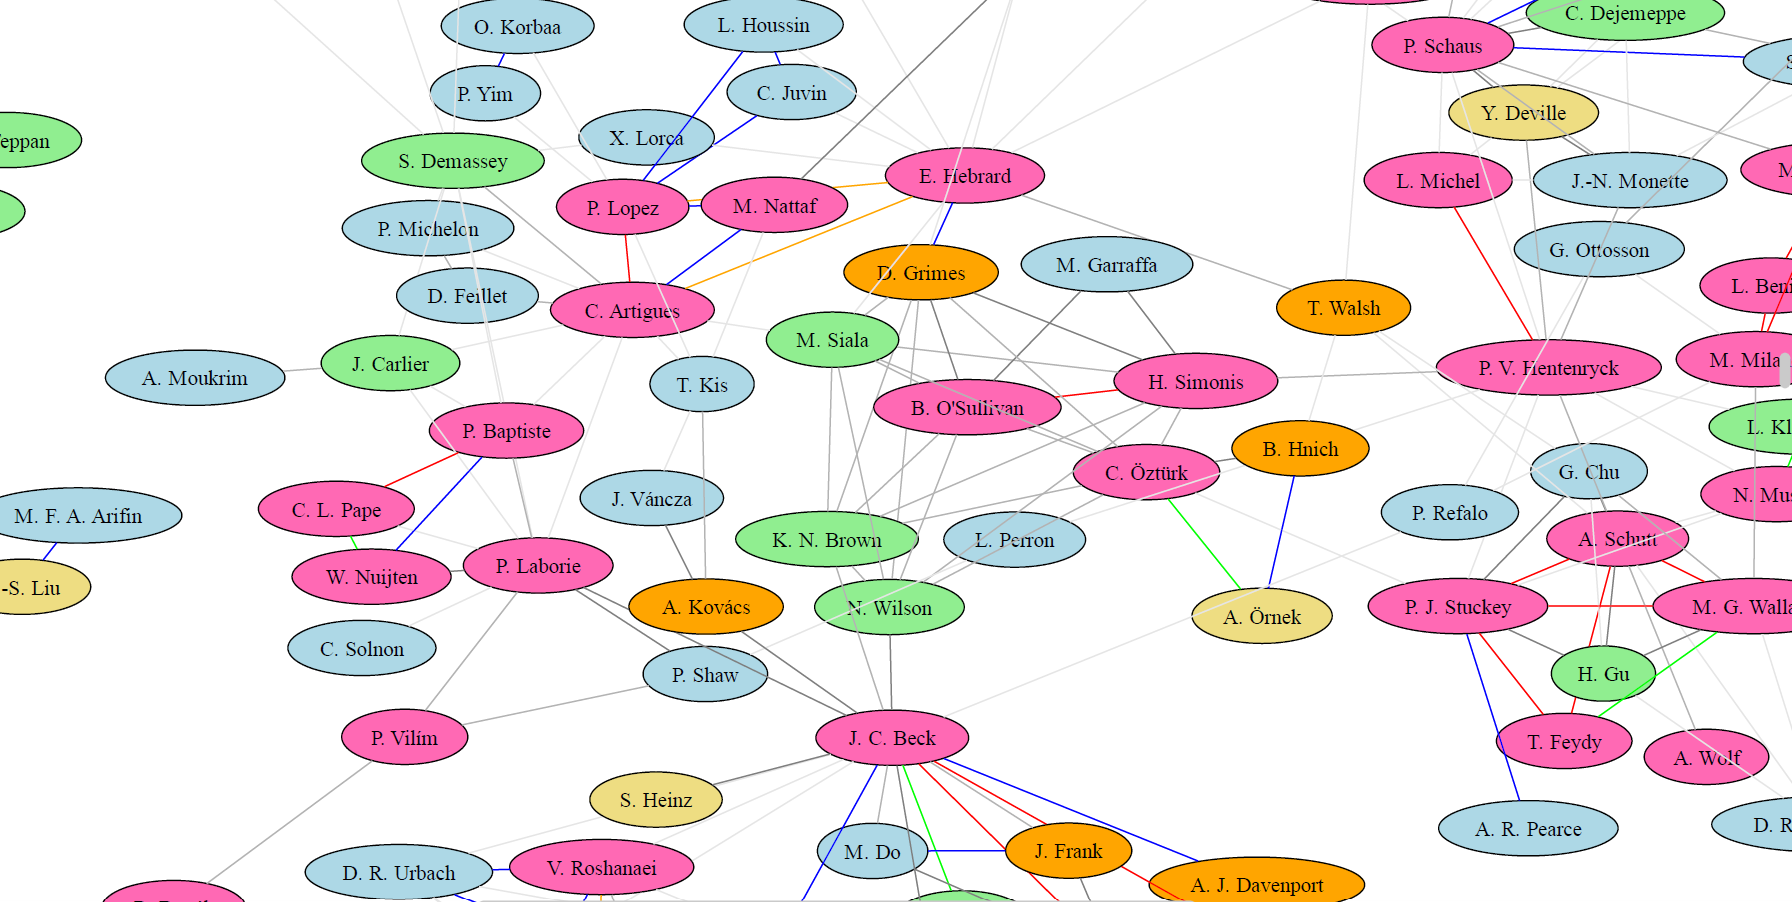
\includegraphics[width=11cm]{images/schedulingcoauthorgraph}
\end{frame}

\begin{frame}
\frametitle{CP \& Scheduling Concept Matching}
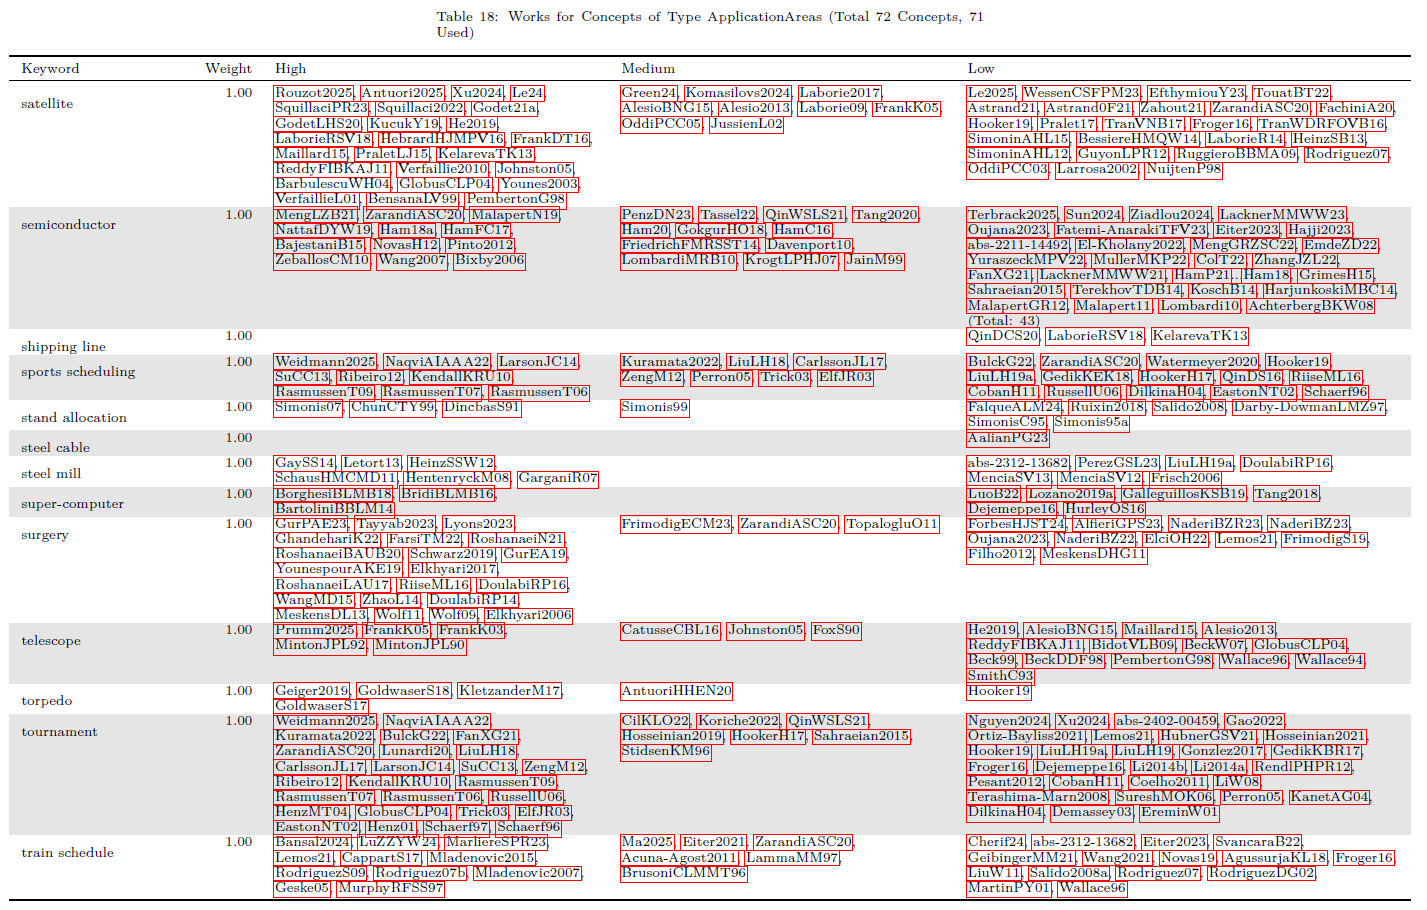
\includegraphics[width=12cm]{images/schedulingconcepts}
\end{frame}



